\section{Introduction}

\subsection{Elastic Rebound Theory and Earthquake Cycles on Transform Faults}

\begin{itemize}
    \item Application of elastic rebound theory and seismic gap hypotheses to stress accumulation and release along fault boundaries.
    \item Shortcommings of the elastic rebound theory in explaining complex earthquake cycles, especially on oceanic transform faults.
\end{itemize}

\subsection{Seismotectonic Setting of our study area and the fault structure}
\begin{itemize}
    \item Tectonic framework of the plate boundary, quasi-periodic seismicity, fault strike, and plate motion. (strike/dip/rake, slip rate, etc.)
    \item Structural characteristics of the fault plane: non-vertical, complex geometry.
    \item Overview of the 2015 and 2025 earthquake sequence occurring along the same fault system within a 10-year span as shown in the figure~\ref{fig: Charlie_Gibbs_seismicity}
\end{itemize}
\begin{figure}[H]
    \centering
    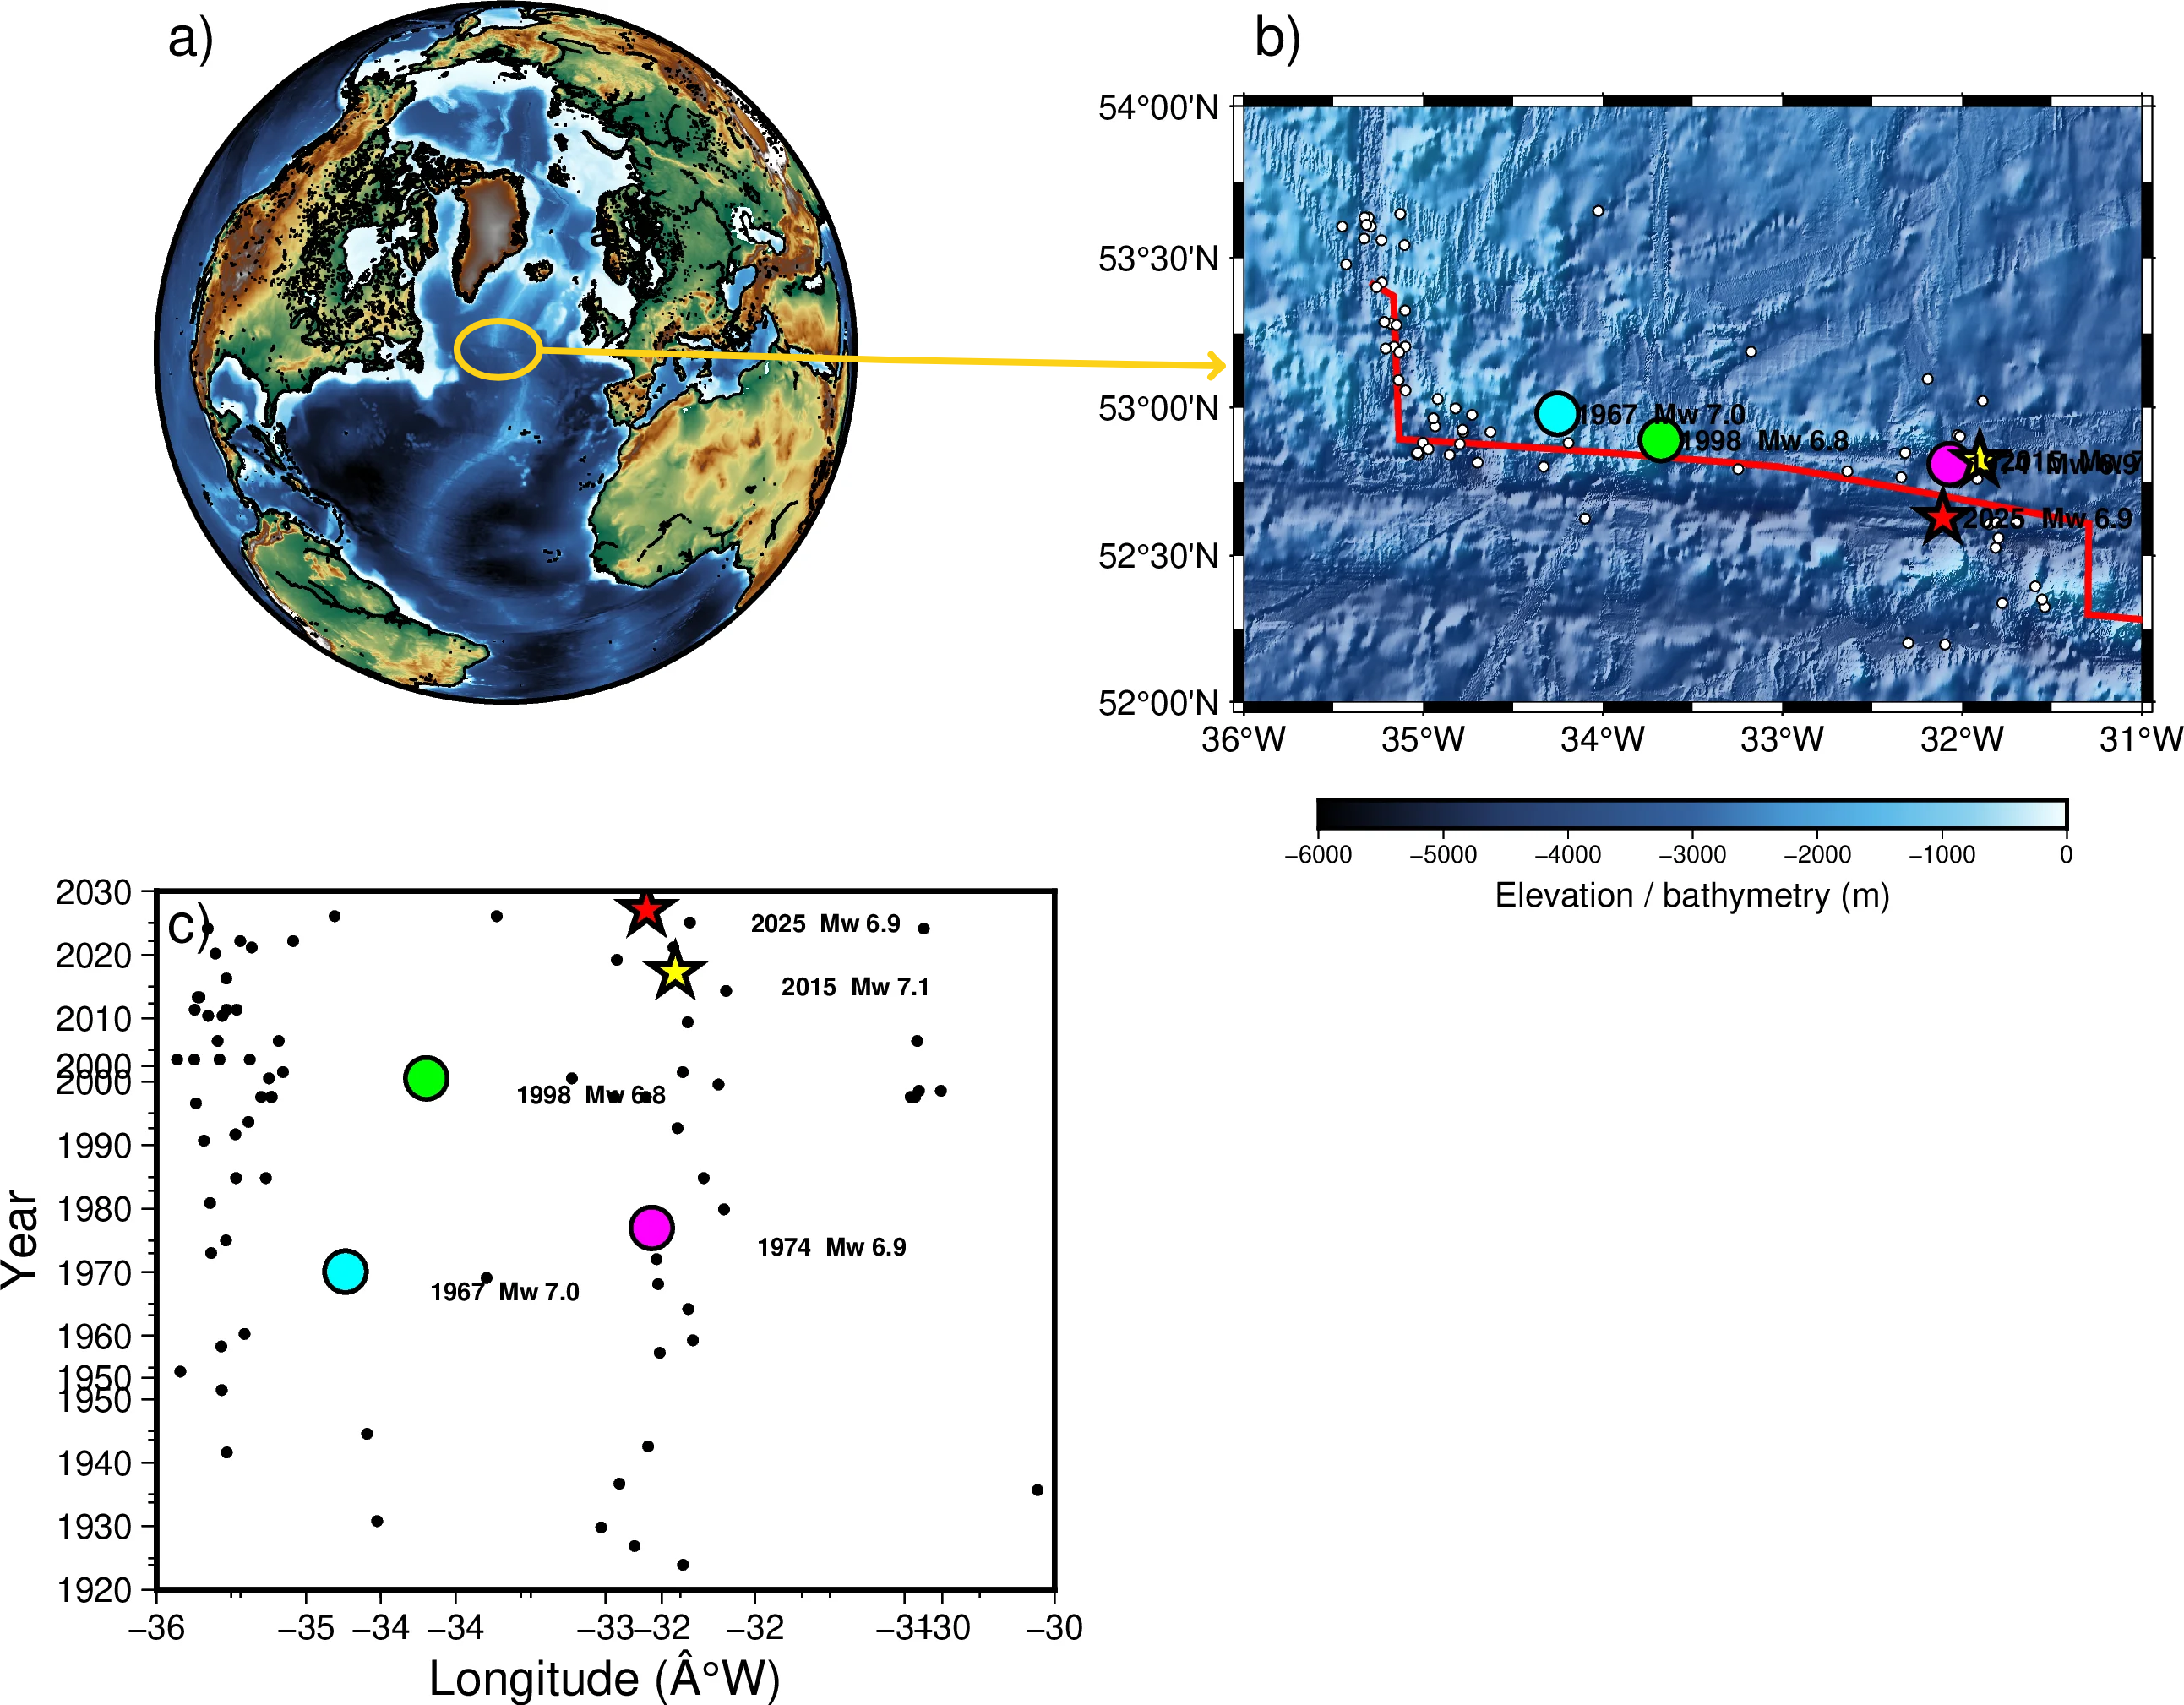
\includegraphics[width=0.79\textwidth]{diagrams/Charlie_Gibbs_seismicity-mh.png}
    \caption{
    Seismicity and tectonic setting of the northern Charlie--Gibbs transform fault.
    (a) Regional tectonic setting shown on a global bathymetric map derived from
    the GMT Earth Relief dataset.
    (b) Detailed bathymetric map of the northern Charlie--Gibbs transform fault,
    based on the 3-arc-sec GMT Earth Relief grid (SRTM3S), with the fault trace
    shown as a solid line refering from \cite{Aderhold2016}. Earthquake epicenters are from
    USGS ComCat, with magnitudes compiled from USGS ComCat and historical
    earthquake catalogues where available. Circle sizes scale with earthquake
    magnitude. The 1967 ($M_w$ 7.0), 1974 ($M_w$ 6.9), and 1998 ($M_w$ 6.8)
    earthquakes are shown as colored circles, while the 2015 ($M_w$ 7.1) and
    2025 ($M_w$ 6.9) earthquakes are shown as stars.
    (c) Temporal distribution of earthquakes as a function of longitude,
    illustrating the spatial and temporal recurrence of major earthquakes along
    the Charlie--Gibbs transform fault. Bathymetric data are from GMT Earth
    Relief; the 15-arc-sec regional grid is based on SRTM15+ V2.1 and the
    3-arc-sec detailed grid is based on SRTM3S.
    }
    \label{fig: Charlie_Gibbs_seismicity}
\end{figure}

\subsection{Unresolved Questions and Study Objectives}
\begin{itemize}
    \item As shown in Figure~\ref{fig: Charlie_Gibbs_seismicity}, the 2025 earthquake occurred only about 10 years after the 2015 
    earthquake and affected the same section of the Charlie--Gibbs transform fault. Such a short recurrence interval is not evident 
    in the historical seismicity of the fault (Figure~\ref{fig: Charlie_Gibbs_seismicity}(c)). Given the relatively slow plate motion
     of $\sim$2.24~cm/yr \cite{DeMets1990}, only about 22~cm of tectonic displacement would accumulate over 10 years. This is much 
     smaller than the several metres of slip typically associated with a large earthquake. The occurrence of two large earthquakes 
     on the same fault segment within such a short time interval is therefore unexpected in the framework of a simple stress-loading 
     and elastic-rebound model, where a major earthquake is expected to release accumulated strain and consequently delay another 
     large rupture on the same segment.
    \item To investigate: Are the slip distributions of the 2015 and 2025 earthquakes similar or different? If different, what are the implications for stress accumulation and release along the fault system?
\end{itemize}
...